\documentclass[fleqn]{article}

\usepackage[utf8]{inputenc}
\usepackage{amsmath}
\usepackage{graphicx}
\usepackage{bm}
\usepackage[margin=0.75in]{geometry}
\usepackage{indentfirst}

\newcommand*\diff{\mathop{}\!\mathrm{d}}
\newcommand*\Diff[1]{\mathop{}\!\mathrm{d^#1}}
\newcommand{\cnum}{ECE 141 COVID-19 Project}
\newcommand{\ced}{Spring 2020}

\begin{document}

\title{ECE 141 COVID-19 Project}
\author{Comran Morshed (SID: 404544982, Discussion 1D)}
\date{}
\maketitle

\section*{Problem 1}
Based on the results of the simulation (shown below), it appears that an overwhelming majority of the population became infected -- causing about 14\% of people to die. There also appears to be a peak infection that is quickly reached around $t=25$, which ultimately decays as more individuals settle into either the recovered or dead group.

\begin{center}
    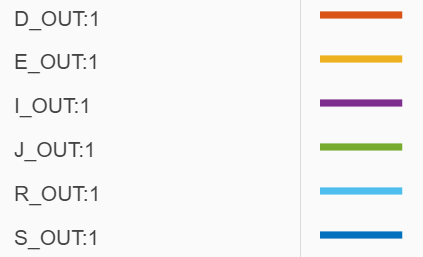
\includegraphics[width=4cm]{outbreak_legend} \\
    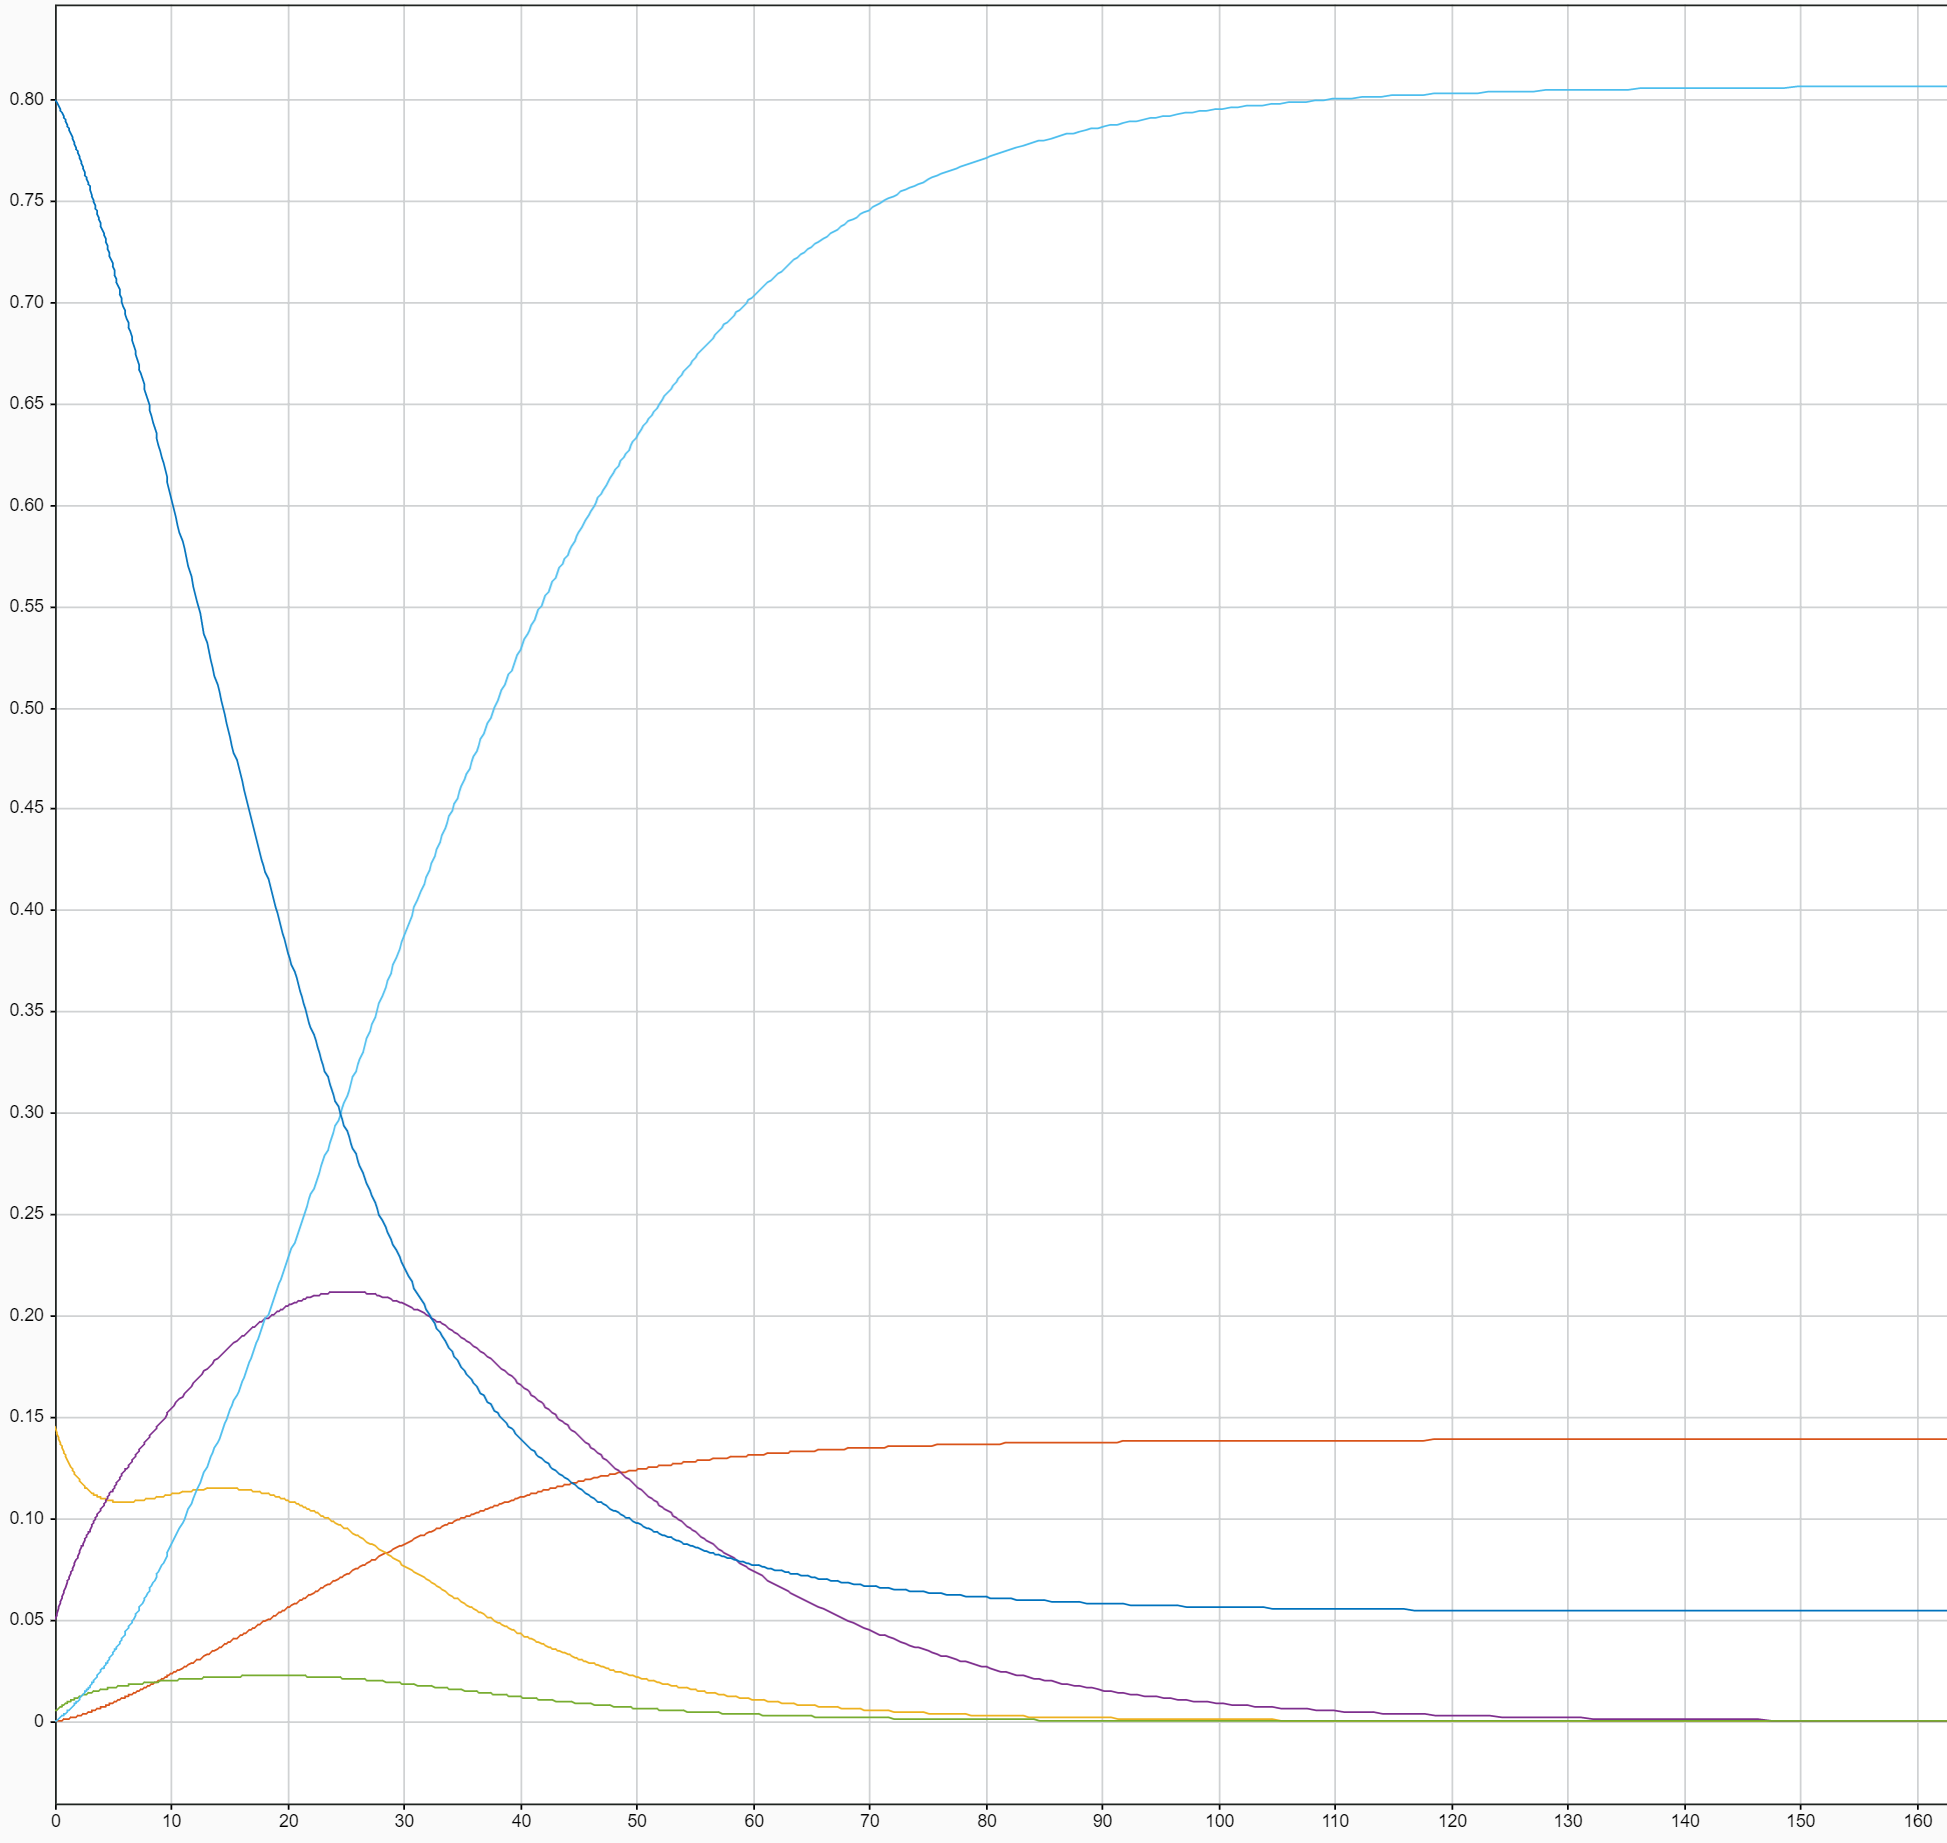
\includegraphics[width=0.85\linewidth]{outbreak_graph}
\end{center}

\newpage

\subsection*{Nonlinear Laplace transforms}
\noindent
$sS(s) = -\beta_1 S I(s) - \beta_2 S J(s) + S(0)$ \\
$sE(s) = \beta_1 S I(s) + \beta_2 S J(s) - \gamma E(s) + E(0)$ \\
$sI(s) = \sigma_1 \gamma E(s) - \rho_1 I(s) + I(0)$ \\
$sJ(s) = \sigma_2 \gamma E(s) - (\rho_2 + q) J(s) + J(0)$ \\
$sR(s) = \rho_1 I(s) + \rho_2 J(s) + R(0)$ \\
$sD(s) = qJ(s) + D(0)$ \\

\subsection*{Simulink diagram for nonlinear model}
\begin{center}
    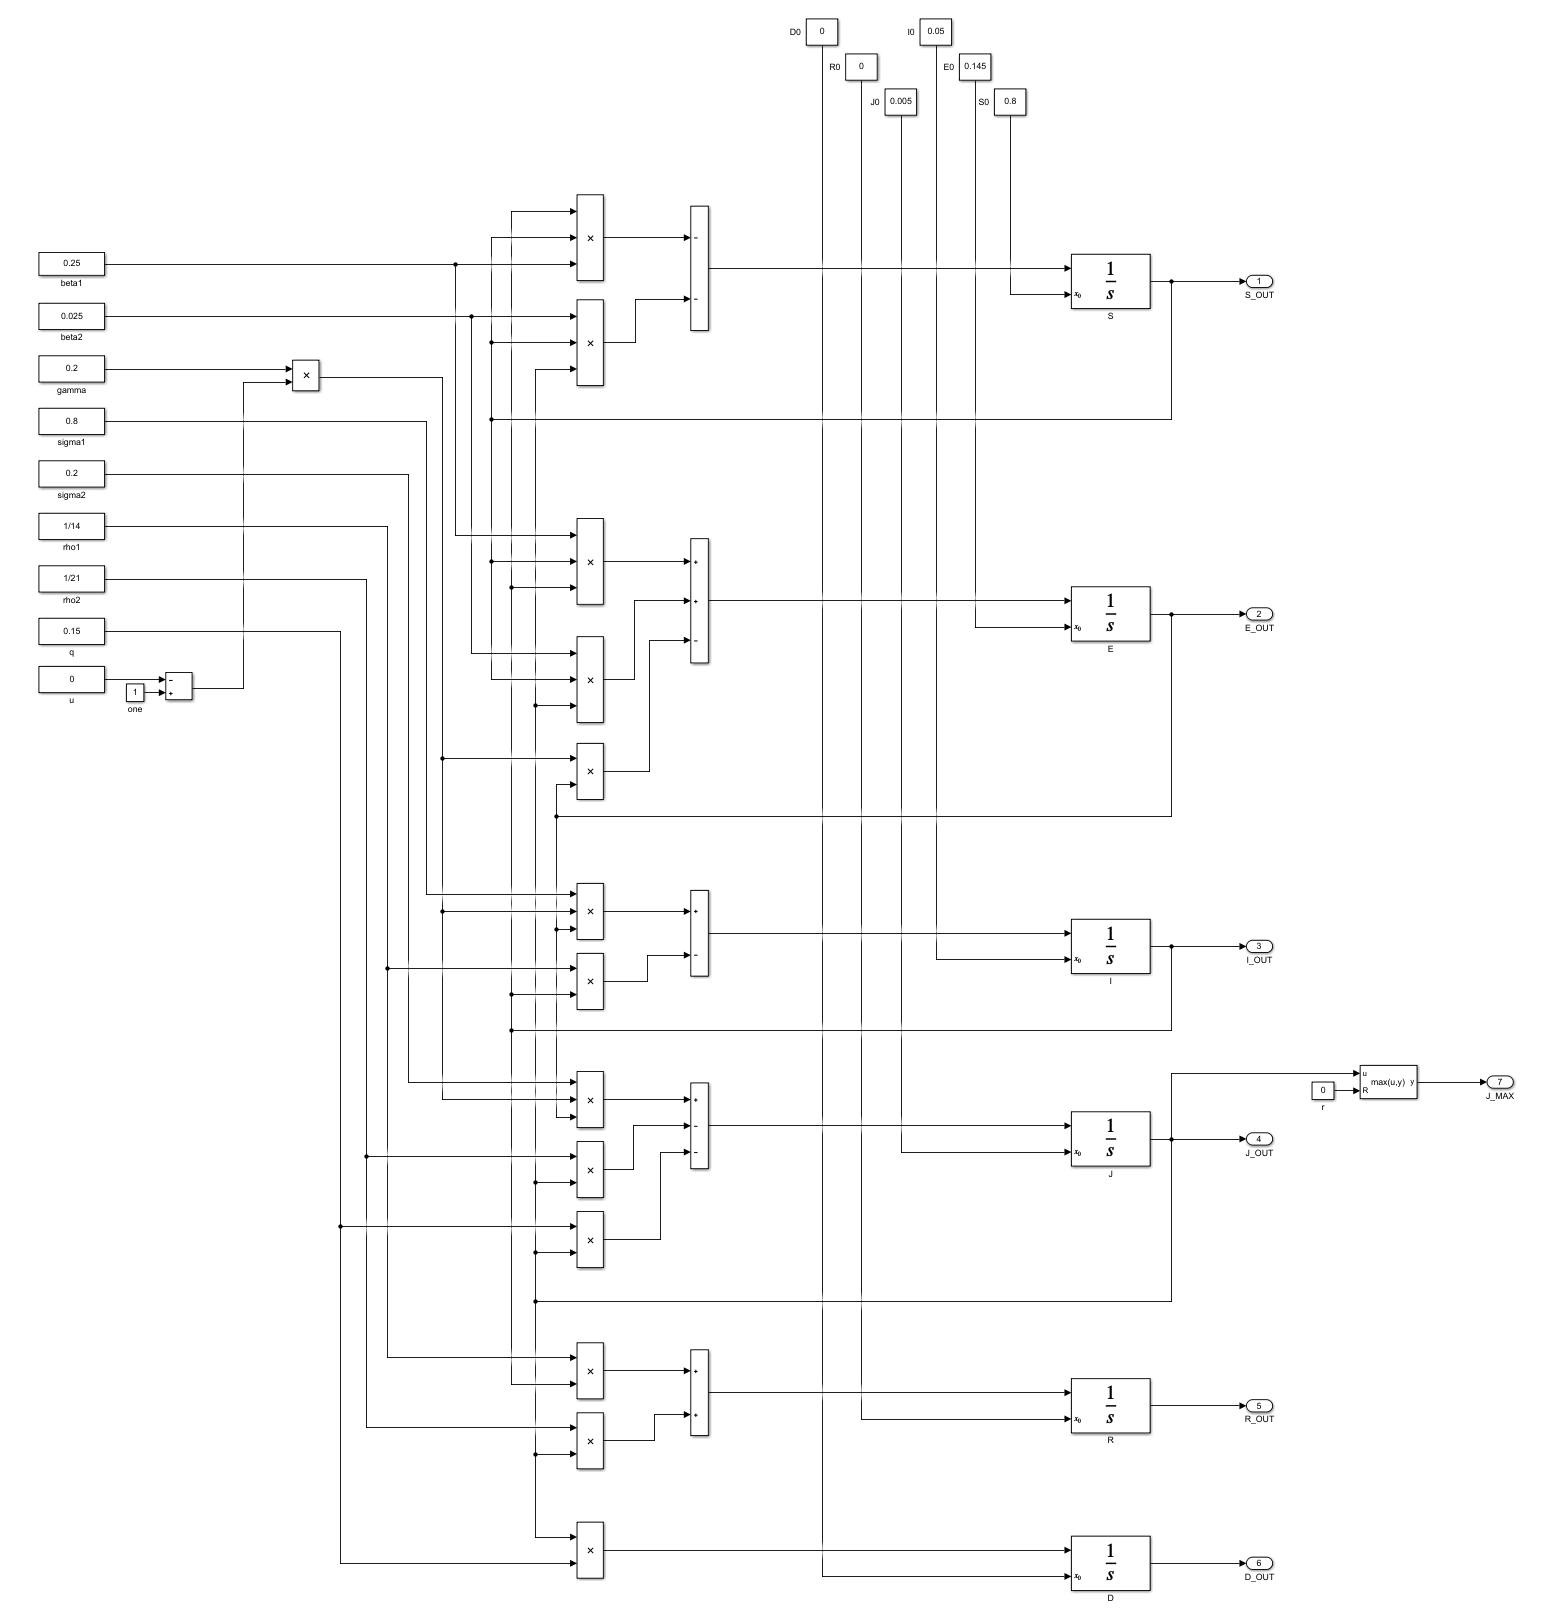
\includegraphics[width=\linewidth]{simulink_diagram}
\end{center}

\newpage

\section*{Problem 2}
There will need to be enough hospital beds to support \textbf{2.25\%} of the population at the peak of the outbreak. This was determined by creating a new signal containing the maximum value of individuals that are seriously ill, and checking the maximum value after the simulation has reached steady state. This is more than twice the percentage of hospital beds available for this population, so there will ultimately be seriously ill individuals who cannot be treated by the overwhelmed hospital system (which, in addition, may have an even lower treatment capabilities as doctors and nurses also become infected).
\begin{center}
    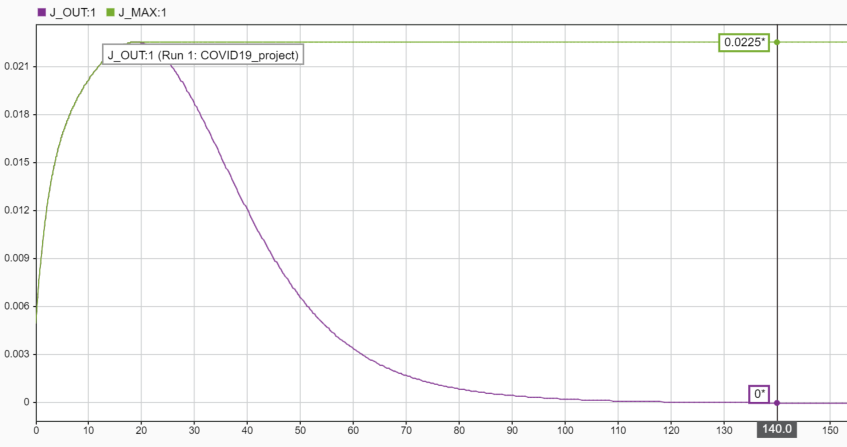
\includegraphics[width=\linewidth]{simulink_J_max}
\end{center}

\newpage
\section*{Problem 3}
\subsection*{Linearization}
\begin{equation*}
    \bm{x} = \begin{bmatrix}
        x_1 \\
        x_2 \\
        x_3 \\
        x_4 \\
        x_5 \\
        x_6
    \end{bmatrix} = \begin{bmatrix}
        S \\
        E \\
        I \\
        J \\
        R \\
        D
    \end{bmatrix}
\end{equation*}

\begin{equation*}
    A = \dfrac{\diff f}{\diff x} \bigg\rvert_{\bm{x_e}, \bm{u_e}}
\end{equation*}

\begin{equation*}
    B = \dfrac{\diff f}{\diff u} \bigg\rvert_{\bm{x_e}, \bm{u_e}}
\end{equation*}

Plug in the model used for this project.

\begin{equation*}
    \begin{split}
        \dfrac{\diff}{\diff t} \diff x & = \bm{A} \diff x + \bm{B} \diff u \bigg\rvert_{\bm{x_e}, \bm{u_e}} \\
            & = \begin{bmatrix}
                0 & 0 & {-\beta_1 S_e} & {-\beta_2 S_e} & 0 & 0 \\
                0 & -(1 - u_e) \gamma & {\beta_1 S_e} & {\beta_2 S_e} & 0 & 0 \\
                0 & (1 - u_e) \sigma_1 \gamma & -\rho_1 & 0 & 0 & 0 \\
                0 & (1 - u_e) \sigma_2 \gamma & 0 & -(\rho_2 + q) & 0 & 0 \\
                0 & 0 & \rho_1 & \rho_2 & 0 & 0 \\
                0 & 0 & 0 & q & 0 & 0 \\
            \end{bmatrix} \cdot \begin{bmatrix}
                \diff S \\
                \diff E \\
                \diff I \\
                \diff J \\
                \diff R \\
                \diff D
            \end{bmatrix} + \begin{bmatrix}
                0 \\
                \gamma E_e \\
                -\sigma_1 \gamma E_e \\
                -\sigma_q \gamma E_e \\
                0 \\
                0
            \end{bmatrix} \diff u
    \end{split}
\end{equation*}


\subsection*{Equilibrium pair}
Need to find an equilibrium pair s.t. $f(x_e, u_e) = 0$.

\begin{equation*}
    \begin{split}
        \begin{bmatrix}
            0 \\
            0 \\
            0 \\
            0 \\
            0 \\
            0 \\
        \end{bmatrix} & = \begin{bmatrix}
            0 & 0 & {-\beta_1 S_e} & {-\beta_2 S_e} & 0 & 0 \\
            0 & -(1 - u_e) \gamma & {\beta_1 S_e} & {\beta_2 S_e} & 0 & 0 \\
            0 & (1 - u_e) \sigma_1 \gamma & -\rho_1 & 0 & 0 & 0 \\
            0 & (1 - u_e) \sigma_2 \gamma & 0 & -(\rho_2 + q) & 0 & 0 \\
            0 & 0 & \rho_1 & \rho_2 & 0 & 0 \\
            0 & 0 & 0 & q & 0 & 0 \\
        \end{bmatrix} \cdot \begin{bmatrix}
            S_e \\
            E_e \\
            I_e \\
            J_e \\
            R_e \\
            D_e
        \end{bmatrix} + \begin{bmatrix}
            0 \\
            \gamma E_e \\
            -\sigma_1 \gamma E_e \\
            -\sigma_q \gamma E_e \\
            0 \\
            0
        \end{bmatrix} u_e \\
        & = \begin{bmatrix}
            0 & 0 & {-\beta_1 S_e} & {-\beta_2 S_e} & 0 & 0 \\
            0 & -(1 - u_e) \gamma & {\beta_1 S_e} & {\beta_2 S_e} & 0 & 0 \\
            0 & (1 - u_e) \sigma_1 \gamma & -\rho_1 & 0 & 0 & 0 \\
            0 & (1 - u_e) \sigma_2 \gamma & 0 & -(\rho_2 + q) & 0 & 0 \\
            0 & 0 & \rho_1 & \rho_2 & 0 & 0 \\
            0 & 0 & 0 & q & 0 & 0 \\
        \end{bmatrix} \cdot \begin{bmatrix}
            S_e \\
            0 \\
            0 \\
            0 \\
            R_e \\
            D_e
        \end{bmatrix} + \begin{bmatrix}
            0 \\
            \gamma \cdot 0 \\
            -\sigma_1 \gamma \cdot 0 \\
            -\sigma_q \gamma \cdot 0 \\
            0 \\
            0
        \end{bmatrix} \cdot u_e
    \end{split}
\end{equation*}

Therefore,
\begin{equation*}
    \begin{bmatrix}
        S_e \\
        E_e \\
        I_e \\
        J_e \\
        R_e \\
        D_e
    \end{bmatrix} = \begin{bmatrix}
        S_e \\
        0 \\
        0 \\
        0 \\
        R_e \\
        D_e
    \end{bmatrix}
\end{equation*}

\subsection*{Final linearized form}
\begin{equation*}
    \dfrac{\diff x}{\diff t} = \begin{bmatrix}
        0 & 0 & {-\beta_1 S_e} & {-\beta_2 S_e} & 0 & 0 \\
        0 & -(1 - u_e) \gamma & {\beta_1 S_e} & {\beta_2 S_e} & 0 & 0 \\
        0 & (1 - u_e) \sigma_1 \gamma & -\rho_1 & 0 & 0 & 0 \\
        0 & (1 - u_e) \sigma_2 \gamma & 0 & -(\rho_2 + q) & 0 & 0 \\
        0 & 0 & \rho_1 & \rho_2 & 0 & 0 \\
        0 & 0 & 0 & q & 0 & 0 \\
    \end{bmatrix} \cdot \begin{bmatrix}
        \diff S \\
        \diff E \\
        \diff I \\
        \diff J \\
        \diff R \\
        \diff D
    \end{bmatrix} + \begin{bmatrix}
        0 \\
        0 \\
        0 \\
        0 \\
        0 \\
        0
    \end{bmatrix} \diff u
\end{equation*}

\begin{equation*}
    \bm{A} = \begin{bmatrix}
        0 & 0 & {-\beta_1 S_e} & {-\beta_2 S_e} & 0 & 0 \\
        0 & -(1 - u_e) \gamma & {\beta_1 S_e} & {\beta_2 S_e} & 0 & 0 \\
        0 & (1 - u_e) \sigma_1 \gamma & -\rho_1 & 0 & 0 & 0 \\
        0 & (1 - u_e) \sigma_2 \gamma & 0 & -(\rho_2 + q) & 0 & 0 \\
        0 & 0 & \rho_1 & \rho_2 & 0 & 0 \\
        0 & 0 & 0 & q & 0 & 0 \\
    \end{bmatrix}
\end{equation*}

\begin{equation*}
    \bm{B} = \begin{bmatrix}
        0 \\
        0 \\
        0 \\
        0 \\
        0 \\
        0
    \end{bmatrix}
\end{equation*}

Pick equilibrium values that are expected at the end of the pandemic.
\begin{equation*}
    \begin{bmatrix}
        S_e \\
        R_e \\
        D_e
    \end{bmatrix} = \begin{bmatrix}
        0.0542 \\
        0.807 \\
        0.139
    \end{bmatrix}
\end{equation*}

\begin{equation*}
    u_e = 0
\end{equation*}

\subsection*{Linear Laplace transforms}
\noindent
$sS(s) = -\beta_1 S_e I(s) - \beta_2 S_e J(s) + S(0)$ \\
$sE(s) = \beta_1 S_e I(s) + \beta_2 S_e J(s) - (1-u_e) \gamma E(s) + E(0)$ \\
$sI(s) = (1-u_e) \sigma_1 \gamma E(s) - \rho_1 I(s) + I(0)$ \\
$sJ(s) = (1-u_e) \sigma_2 \gamma E(s) - (\rho_2 + q) J(s) + J(0)$ \\
$sR(s) = \rho_1 I(s) + \rho_2 J(s) + R(0)$ \\
$sD(s) = qJ(s) + D(0)$ \\

\newpage

\subsection*{Linearized simulation}
\begin{center}
    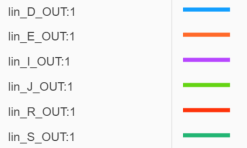
\includegraphics[width=4cm]{linear_outbreak_legend} \\
    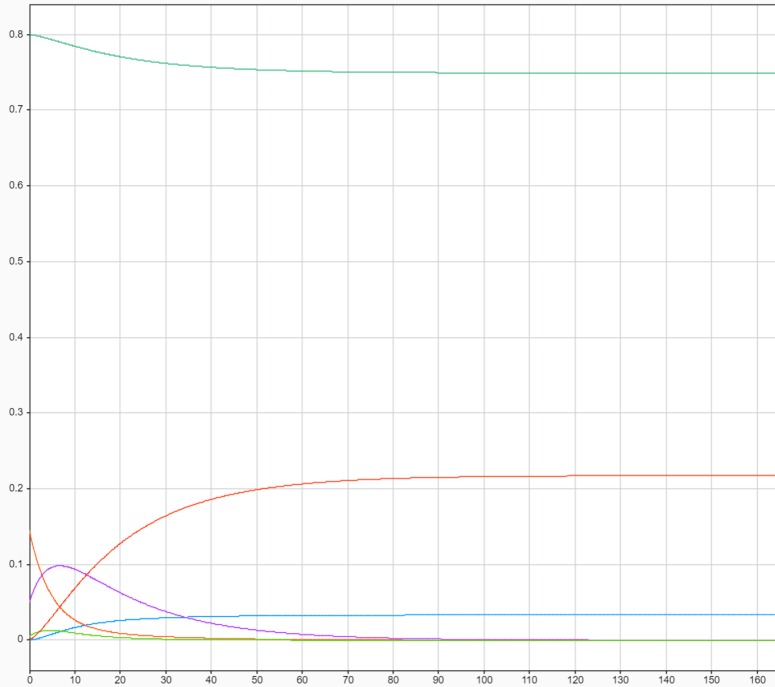
\includegraphics[width=0.85\linewidth]{linear_outbreak_graph}
\end{center}

\newpage

\subsection*{Simulink diagram for linear model}
\begin{center}
    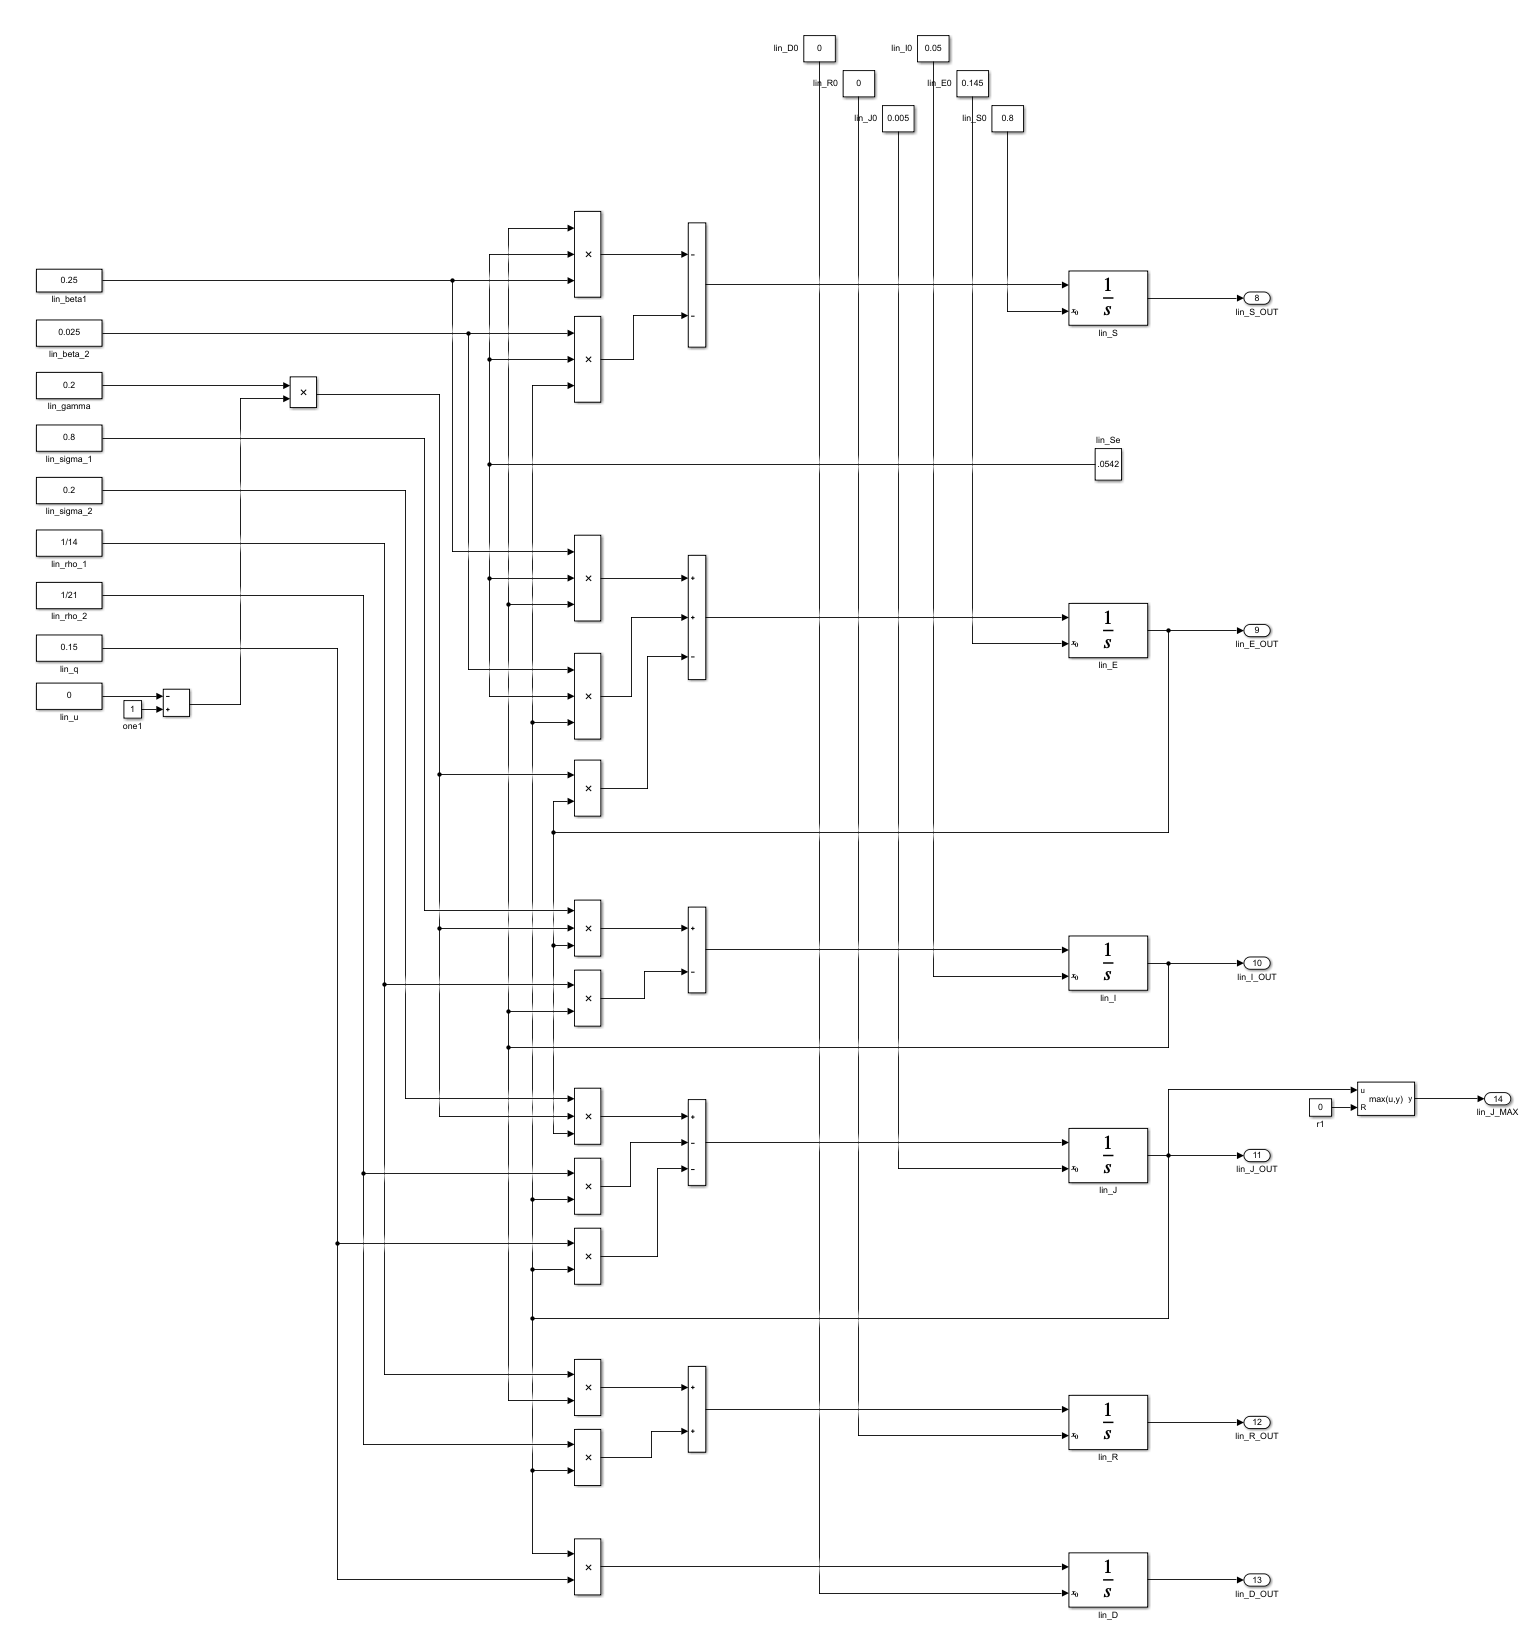
\includegraphics[width=\linewidth]{linear_simulink_diagram}
\end{center}

\subsection*{Issue with the linearized model}
This linearized model may not be adequate for control since it assumes a constant value for $S_e$. In reality, this value is much higher at the beginning of the pandemic than at the end as the population becomes immune to the disease. Therefore, the linearized model would deviate from the actual nonlinear model as more time passes by.

\section*{Problem 4}
\subsection*{Find a transfer function from J(0) $\rightarrow$ J}

$sJ(s) = (1-u_e) \sigma_2 \gamma E(s) - (\rho_2 + q) J(s) + J(0)$ \\
$J(s)(s + \rho_2 + q) = (1-u_e) \sigma_2 \gamma E(s) + J(0)$ \\
$J(s) = \dfrac{(1-u_e) \sigma_2 \gamma E(s) + J(0)}{s + \rho_2 + q}$ \\
$J(s) = \dfrac{(1-u_e) \sigma_2 \gamma}{s + \rho_2 + q} E(s) + \dfrac{J(0)}{s + \rho_2 + q}$ \\
\\
\\
$sE(s) = \beta_1 S_e I(s) + \beta_2 S_e J(s) - (1-u_e) \gamma E(s) + E(0)$ \\
$E(s)(s + (1-u_e) \gamma) = \beta_1 S_e I(s) + \beta_2 S_e J(s) + E(0)$ \\
\\
$sI(s) = (1-u_e) \sigma_1 \gamma E(s) - \rho_1 I(s) + I(0)$ \\
$I(s)(s + \rho_1) = (1-u_e) \sigma_1 \gamma E(s) + I(0)$ \\
$I(s) = \dfrac{(1-u_e) \sigma_1 \gamma E(s) + I(0)}{s + \rho_1}$ \\
\\
\\
Set $E(0) = 0$, $I(0) = 0$: \\
$E(s)(s + (1-u_e) \gamma) = \dfrac{\beta_1 \sigma_1 \gamma S_e (1-u_e)}{s + \rho_1} E(s) + \beta_2 S_e J(s)$ \\
$E(s)\left(s + (1-u_e) \gamma - \dfrac{\beta_1 \sigma_1 \gamma S_e (1-u_e)}{s + \rho_1}\right) = \beta_2 S_e J(s)$ \\
$E(s) = \dfrac{\beta_2 S_e (s + \rho_1)}{s (s + \rho_1) + (1-u_e) (s + \rho_1) \gamma - \beta_1 \sigma_1 \gamma S_e (1-u_e)} J(s)$ \\

\begin{equation*}
\begin{split}
J(s) & = \dfrac{(1-u_e) \sigma_2 \gamma}{s + \rho_2 + q} \dfrac{\beta_2 S_e (s + \rho_1)}{s (s + \rho_1) + (1-u_e) (s + \rho_1) \gamma - \beta_1 \sigma_1 \gamma S_e (1-u_e)} J(s) + \dfrac{J(0)}{s + \rho_2 + q} \\
    & = \dfrac{\beta_2 S_e \sigma_2 \gamma (1-u_e)(s + \rho_1)}{s (s + \rho_1) + (1-u_e) (s + \rho_1) \gamma - \beta_1 \sigma_1 \gamma S_e (1-u_e)} J(s) + \dfrac{J(0)}{s + \rho_2 + q}
\end{split}
\end{equation*}

\begin{equation*}
\begin{split}
J(s)\left(1 - \dfrac{\beta_2 S_e \sigma_2 \gamma (1-u_e)(s + \rho_1)}{s (s + \rho_1) + (1-u_e) (s + \rho_1) \gamma - \beta_1 \sigma_1 \gamma S_e (1-u_e)}\right) & = \dfrac{J(0)}{s + \rho_2 + q}
\end{split}
\end{equation*}

\begin{equation*}
\begin{split}
\dfrac{J(s)}{J(0)} & = \dfrac{1}{\left(1 - \dfrac{\beta_2 S_e \sigma_2 \gamma (1-u_e)(s + \rho_1)}{s (s + \rho_1) + (1-u_e) (s + \rho_1) \gamma - \beta_1 \sigma_1 \gamma S_e (1-u_e)}\right)(s + \rho_2 + q)} \\
    & = \dfrac{1}{(s + \rho_2 + q) - \dfrac{\beta_2 S_e \sigma_2 \gamma (1-u_e)(s + \rho_1)(s + \rho_2 + q)}{s (s + \rho_1) + (1-u_e) (s + \rho_1) \gamma - \beta_1 \sigma_1 \gamma S_e (1-u_e)}} \\
    & = \dfrac{s (s + \rho_1) + (1-u_e) (s + \rho_1) \gamma - \beta_1 \sigma_1 \gamma S_e (1-u_e)}{(s + \rho_2 + q)(s (s + \rho_1) + (1-u_e) (s + \rho_1) \gamma - \beta_1 \sigma_1 \gamma S_e (1-u_e)) - \beta_2 S_e \sigma_2 \gamma (1-u_e)(s + \rho_1)(s + \rho_2 + q)} \\
    & = \dfrac{s^2 + (\rho_1 + \gamma + \rho_1 \gamma - u_e \gamma - \rho_1 u_e \gamma) s - \beta_1 \sigma_1 \gamma S_e (1-u_e)}{(s + \rho_2 + q)(s^2 + (\rho_1 + \gamma + \rho_1 \gamma - u_e \gamma - \rho_1 u_e \gamma) s - \beta_1 \sigma_1 \gamma S_e (1-u_e) - \beta_2 S_e \sigma_2 \gamma (1-u_e)(s + \rho_1))} \\
    & = \dfrac{s^2 + (0.285714 - 0.214286 u_e)s - 0.002168 (1 - u_e)}{s^3 + (0.468993 - 0.199946 u_e) s^2 + (0.0657426 - 0.0516269 u_e) s + 0.00239393 (1 - u_e)}
\end{split}
\end{equation*}

\newpage

\subsection*{Root locus}
When setting $u_e = 0$, the transfer function has the following root locus:
\begin{center}
    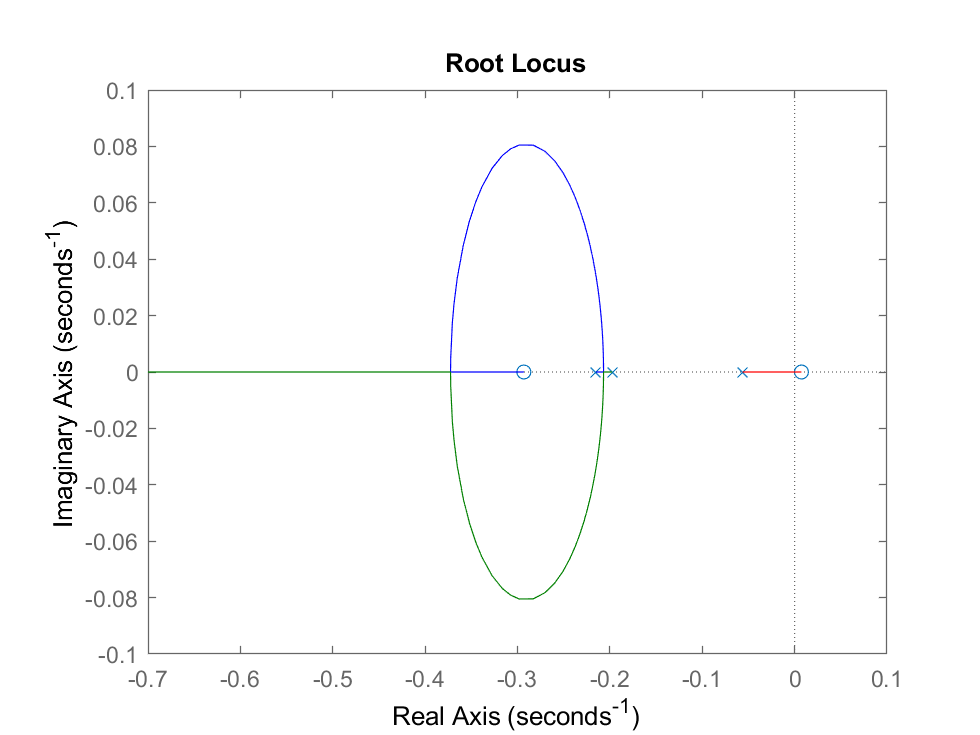
\includegraphics[width=0.7\linewidth]{tf_root_locus_u_0}
\end{center}

Additionally, when setting $u_e = 0.9$, the transfer function has the following root locus:
\begin{center}
    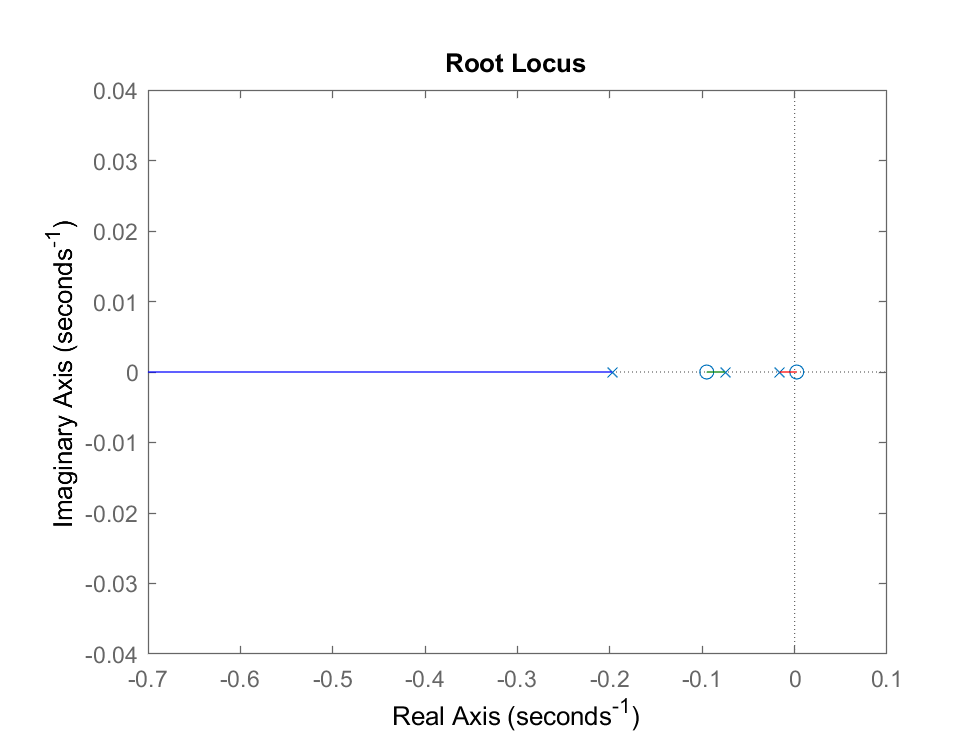
\includegraphics[width=0.7\linewidth]{tf_root_locus_u_0_9}
\end{center}

There are three poles and two zeros in the transfer function, and \textbf{all of the poles/zeros are on the real axis}. In addition, \textbf{higher values of u result in poles that are closer to the imaginary axis}. This would result in a quicker decay of the number of patients requiring critical treatment (classified by variable J) and, therefore, a lower strain on the hospital system. Since wearing masks would logically slow the spread of the disease, it makes intuitive sense that the stress on the hospital system would also decay faster.

\newpage

\section*{Problem 5}
Comparing different values for u in my linear Simulink model supports the conclusion made for this transfer function. In addition, it is apparent that the system shows signs of underdamping for lower values of $u_e$. Although such a system reaches zero sooner, the initial overshoot has the potential to overload the hospital system with critically ill patients. By increasing u, the overshoot begins to disappear and, for the maximal possible value of $u_e = 0.9$, the system begins to resemble a more desirable critically-damped signal.

\begin{center}
    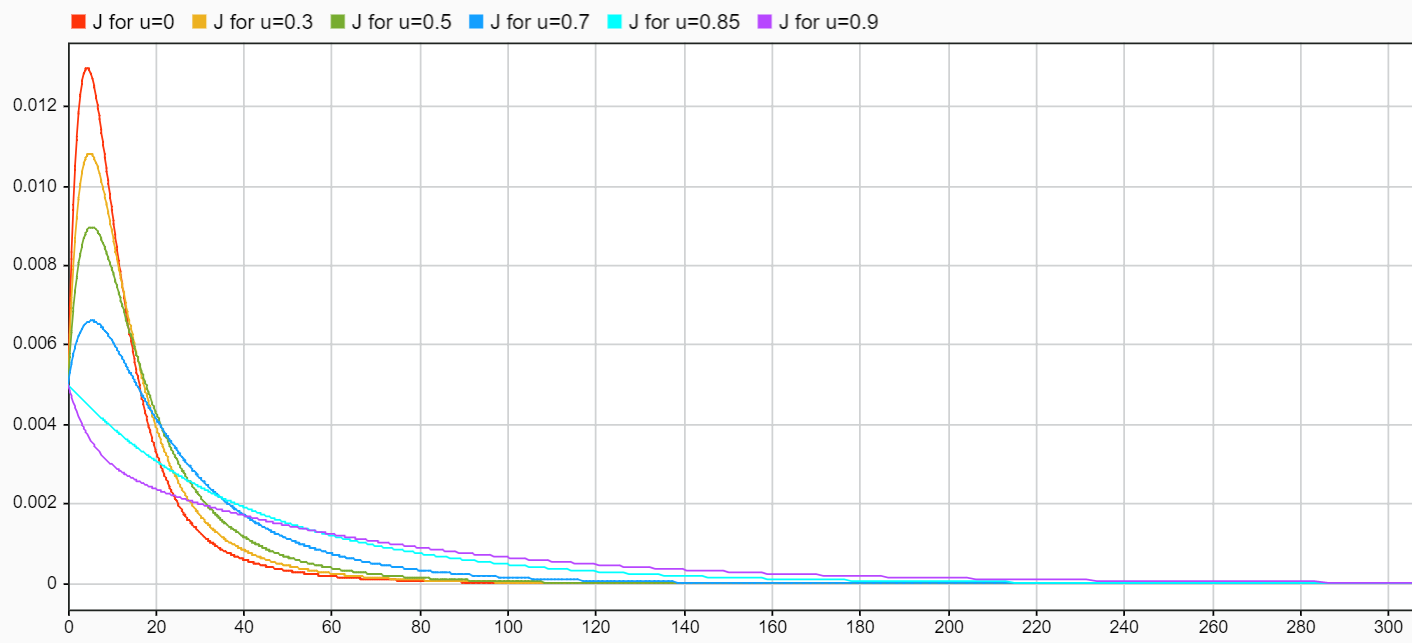
\includegraphics[width=\linewidth]{J_simulink_u_values}
\end{center}

Additionally, the linear model indicates that higher values of u result in a slower decay in the number of susceptible individuals. Again, this makes intuitive sense since masks slow the spread of the disesase through a population.
\begin{center}
    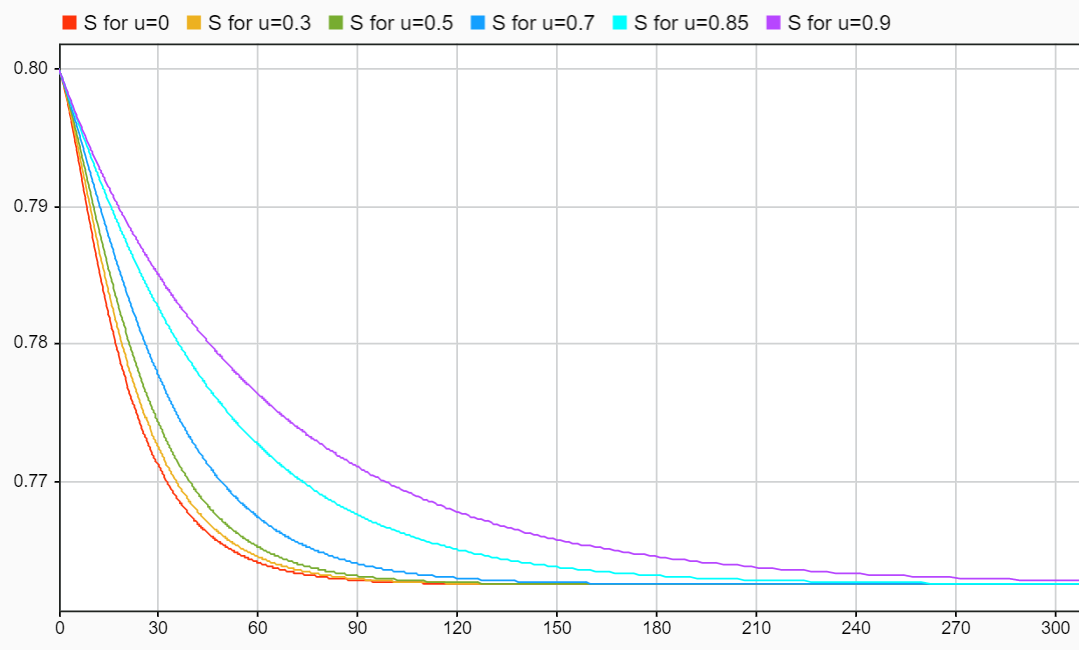
\includegraphics[width=\linewidth]{S_simulink_u_values}
\end{center}

\newpage

Varying the value for u on the nonlinear model shows similar results, with an overall decrease in the maximum overshoot of the signal for critically ill patients. However, the nonlinear model is also able to illustrate a bit of a "lag" for the peak value of J, which does result in the number of hospitalizations going above the initial value ($J(0)$) even for the maximum value of u as more patients become infected.

\begin{center}
    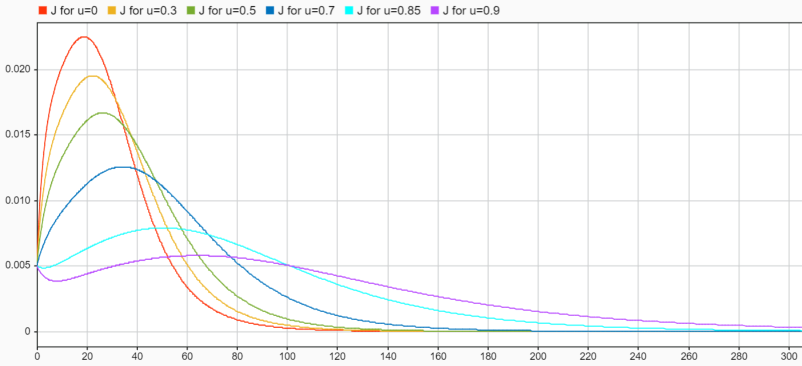
\includegraphics[width=\linewidth]{nonlinear_J_simulink_u_values}
    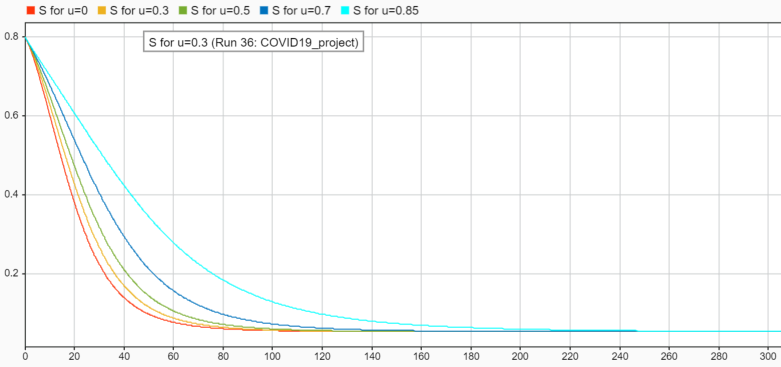
\includegraphics[width=\linewidth]{nonlinear_S_simulink_u_values}
\end{center}

\subsection*{Reason for differences in the linear and nonlinear model}
The linear model is based off of an equilibrium value for S at a specific timestep (in this case, the steady state value at the end of the nonlinear simulation). Therefore, the linear mode appears to have a lower value for the peak hospitalization rates in J. However, given the chosen value for $S_e$, the general shape of the linear and nonlinear models for J are closely related by a constant scalar multiple.

The linear model is also not able to express some of the nuances of the linear model, such as the initial dip in the value for J due to the dependence of E on a dynamic value for S (rather than an equilibrium value). These differences require higher-order degrees of the Taylor series for the nonlinear model to be expressed in a simplified model, so the linearized model effectively disregards them.

\newpage

\section*{Problem 6}
As seen in previous parts, higher values of u result in a more critically damped response in terms of the number of hospitalizations. Therefore, there is less overshoot that can quickly result in an overload of the hospital system. 

\subsection*{Controller design}
With this insight, I designed a controller for the outbreak consisting of distinct mask policies at three timesteps: a strict policy at the beginning of the outbreak, a relaxed policy after the initial spike, and elimination of masks soon after the relaxed policy.

\begin{center}
    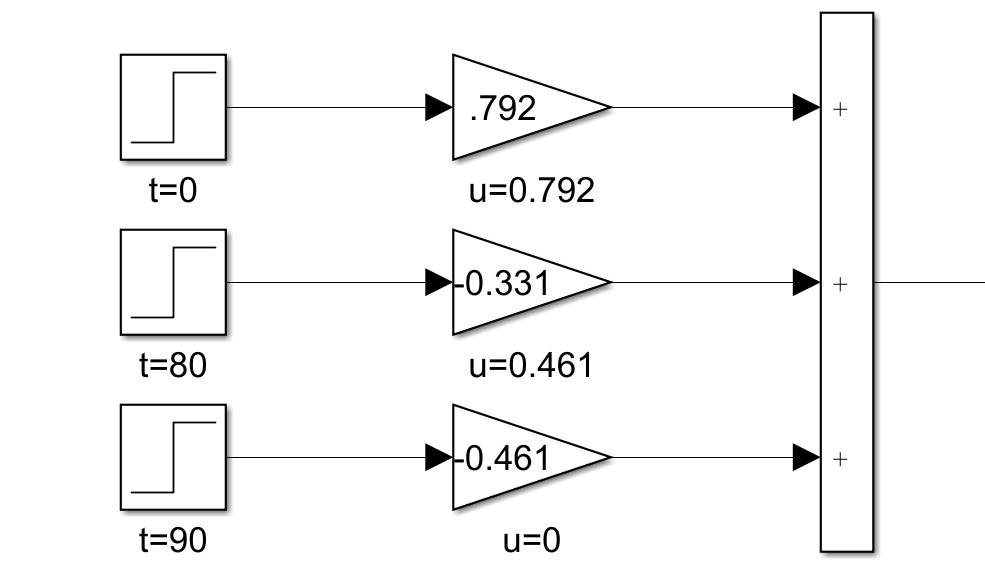
\includegraphics[width=0.5\linewidth]{simulink_mask_policy}
\end{center}

Enforcement of the strict mask policy is critical during early stages of the pandemic beyond \textbf{t=0} since a lower value for u would result in a much higher overshoot in the number of hospitalizations, which is only amplified by the high number of susceptible individuals. However, by \textbf{t=80}, the number of susceptible individuals has decreased to the point where a higher overshoot in hospitalizations is acceptable, and a more relaxed mask policy can be implemented. This relaxed policy also accelerates the decrease of the number of susceptible individuals to the point where the mask policy can be completely eliminated by \textbf{t=90}. 

\subsection*{Simulation results}
Using this controller as an input to the nonlinear model results in a manageable number of hospitalizations throughout the outbreak, with the maximum value for J never exceeding $1\%$.

\begin{center}
    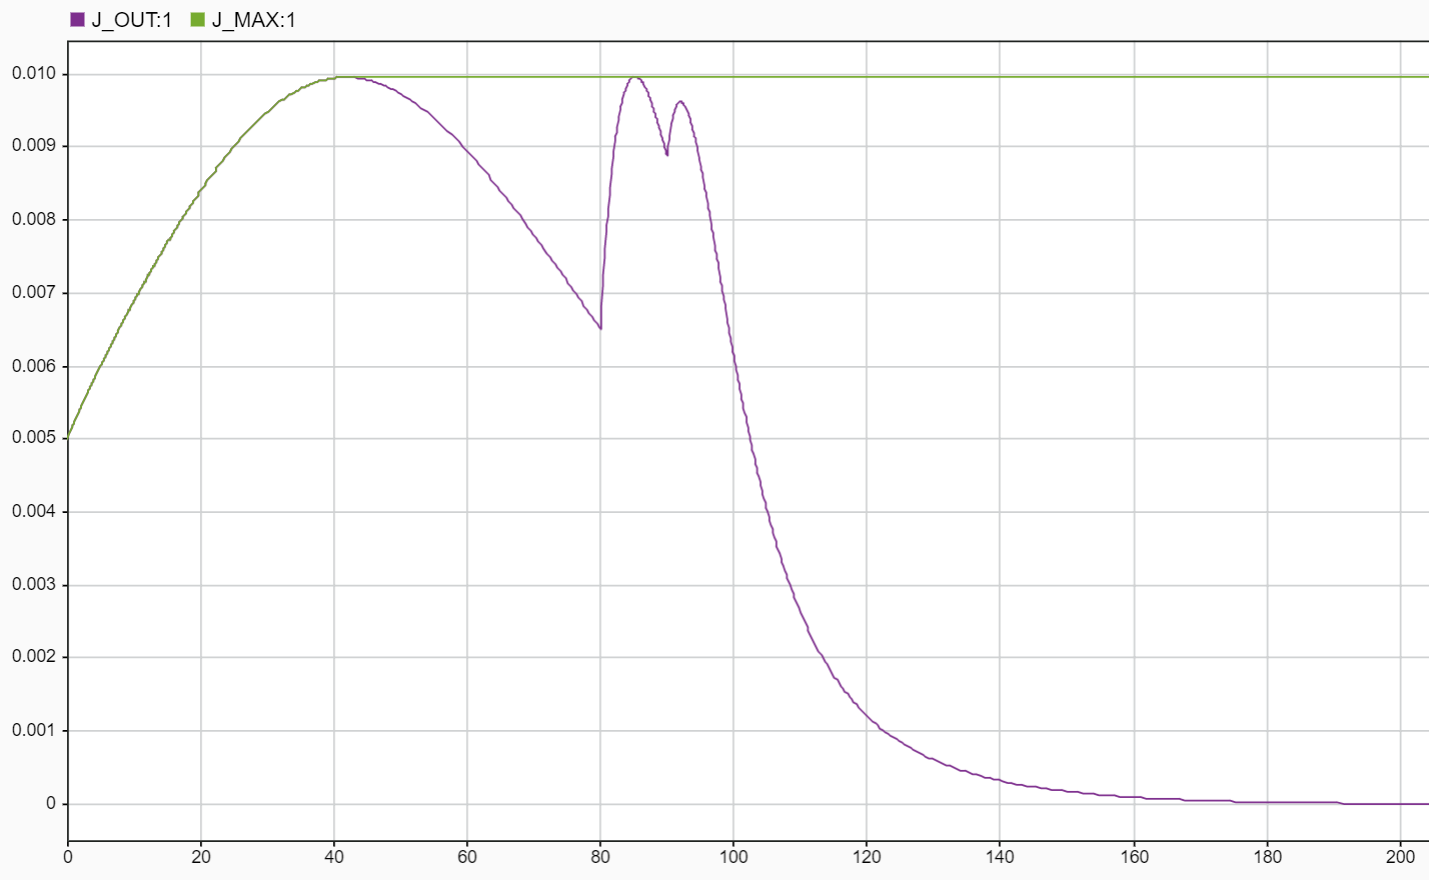
\includegraphics[width=0.8\linewidth]{controlled_outbreak_J_simulink}
\end{center}

\newpage

According to the simulation, this controller for u does not change the number of people who ultimately end up recovering or dying in the outbreak. However, in practice, keeping the number of people who are hospitalized at any given time below $1\%$ is critical to actually seeing the values predicted by this model, and any overload of the hospital system (as shown by my initial model of the outbreak with no mask policy at all) would ultimately result in significantly more deaths as sick individuals are denied treatment due to lack of resources.


\begin{center}
    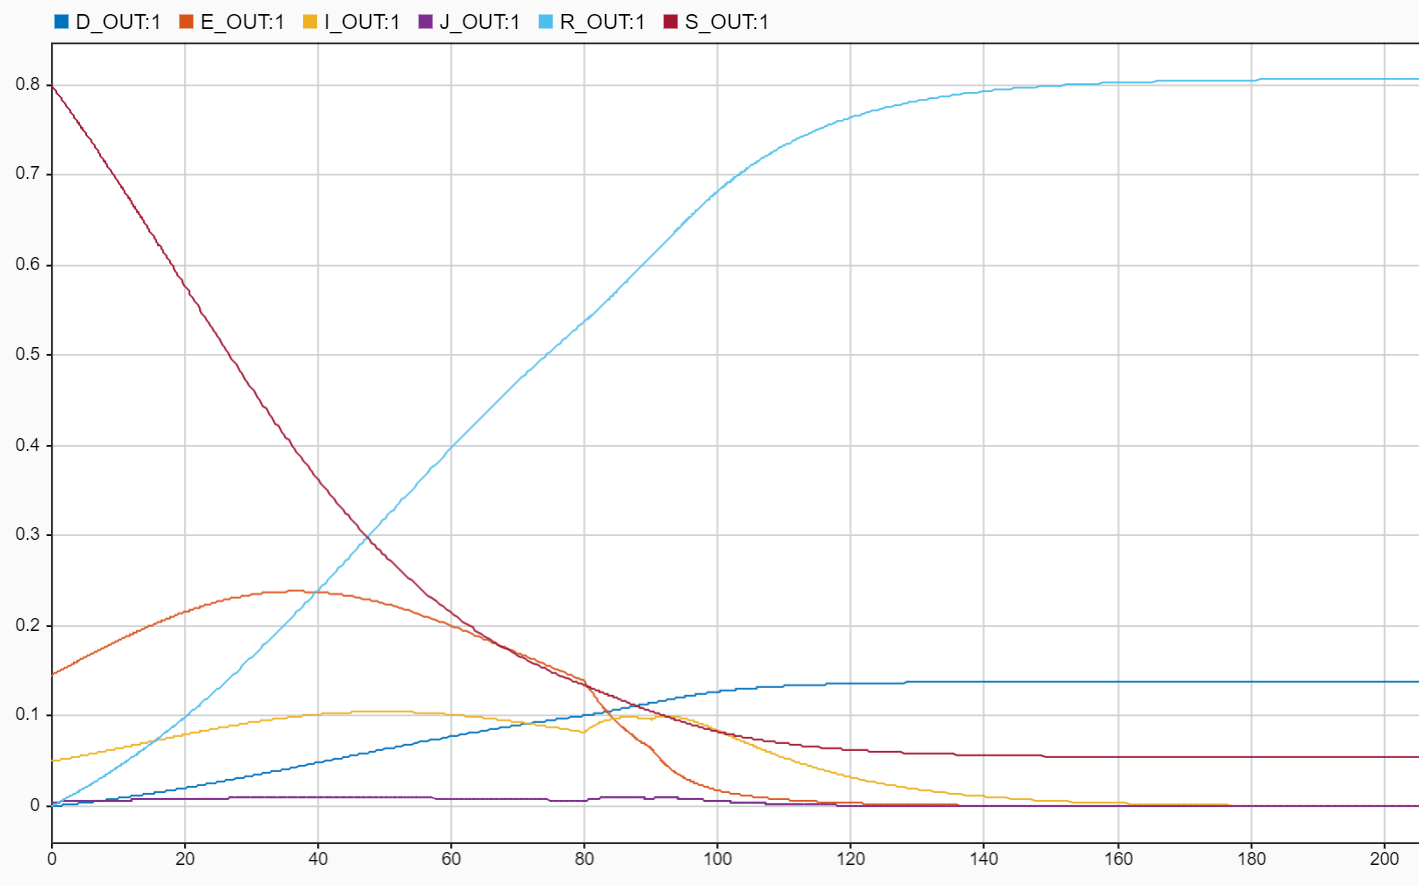
\includegraphics[width=0.8\linewidth]{controlled_outbreak_simulink}
\end{center}

\subsection*{Complete Simulink diagram using the nonlinear model}
\begin{center}
    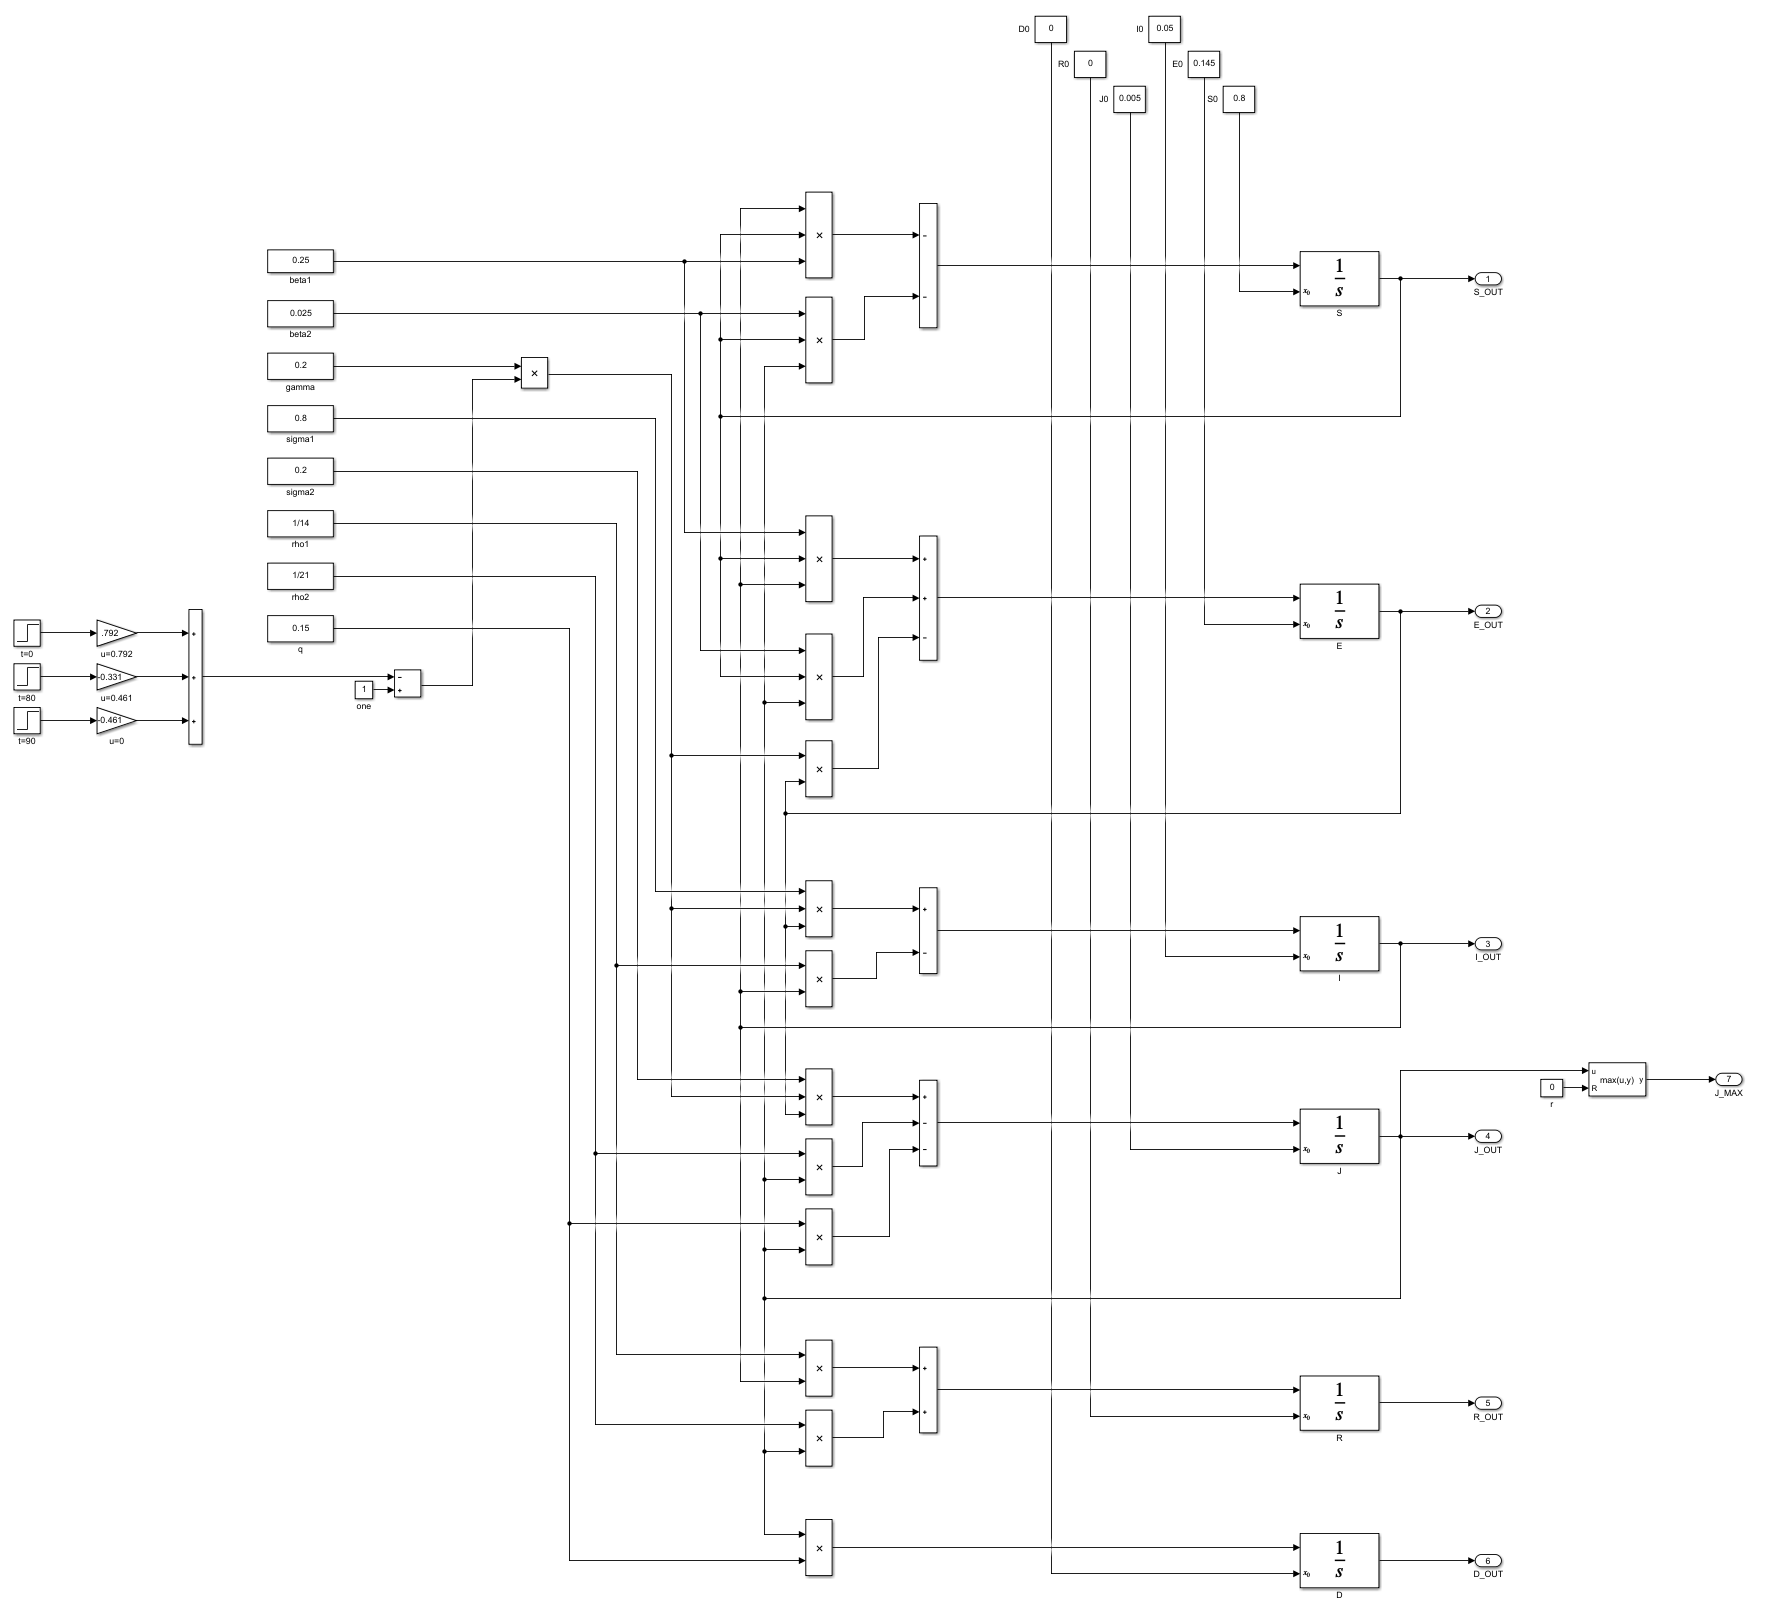
\includegraphics[width=0.7\linewidth]{controlled_simulink}
\end{center}

\section*{Problem 7}
\subsection*{Analysis}
The critical initial conditions for controlling the number of hospitalizations are S, E, I, and J. To analyze the effect of modifying these initial conditions, I used the same controller designed in the previous part to analyze the change in maximum hospitalizations during the outbreak.

Lowering the value of S without disturbing E, I, and J can be accomplished by moving the population to the R and D groups. As far as tuning u, it does not matter whether the population moved all to R or all to D since these terms do not affect the tuning of u. However, a decrease in S ultimately results in a lower maximum value of J since there is already a lower susceptible population that can end up in the hospitalization group. As shown in the following plot where S was decreased by $20\%$, a more relaxed mask policy can be used in this case since there is room for extra overshoot in the model.

\begin{center}
    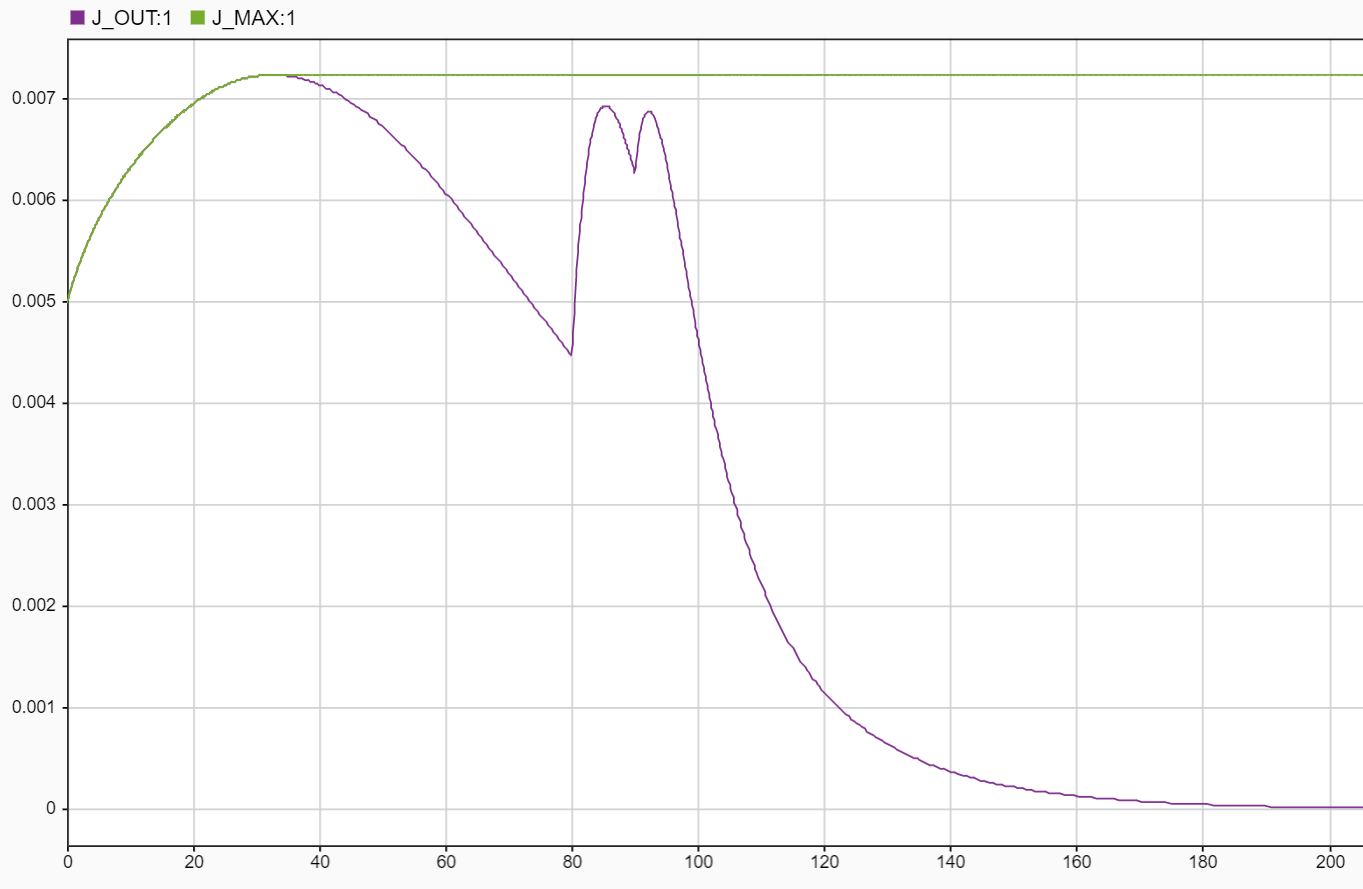
\includegraphics[width=0.7\linewidth]{init_conditions_lower_s}
\end{center}

In contrast, moving $20\%$ of the population from S to E results in a much higher peak value for J since there is a higher initial likelihood of individuals becoming hospitalized since they are already infected with the virus. As shown in the following plot, this situation would require a higher value of u (resulting in a more damped response for J), which can slow the initial hospitalization rate at the beginning of the outbreak to prevent an overload.

\begin{center}
    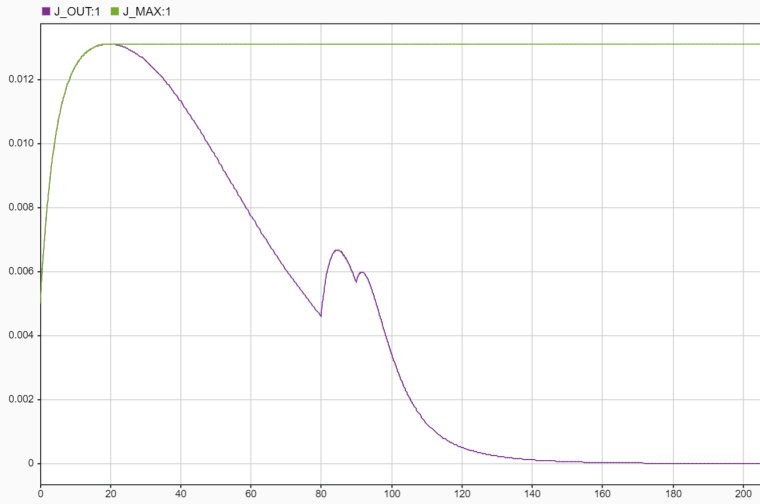
\includegraphics[width=0.7\linewidth]{init_conditions_higher_e}
\end{center}

\newpage

Moving $20\%$ of the population from S to I (representing a higher initial number of infections) results in a bigger initial spike in hospitalizations since infected individuals are quicker to transition into the J group. Therefore, a higher value of u is required to reduce the initial overshoot.

\begin{center}
    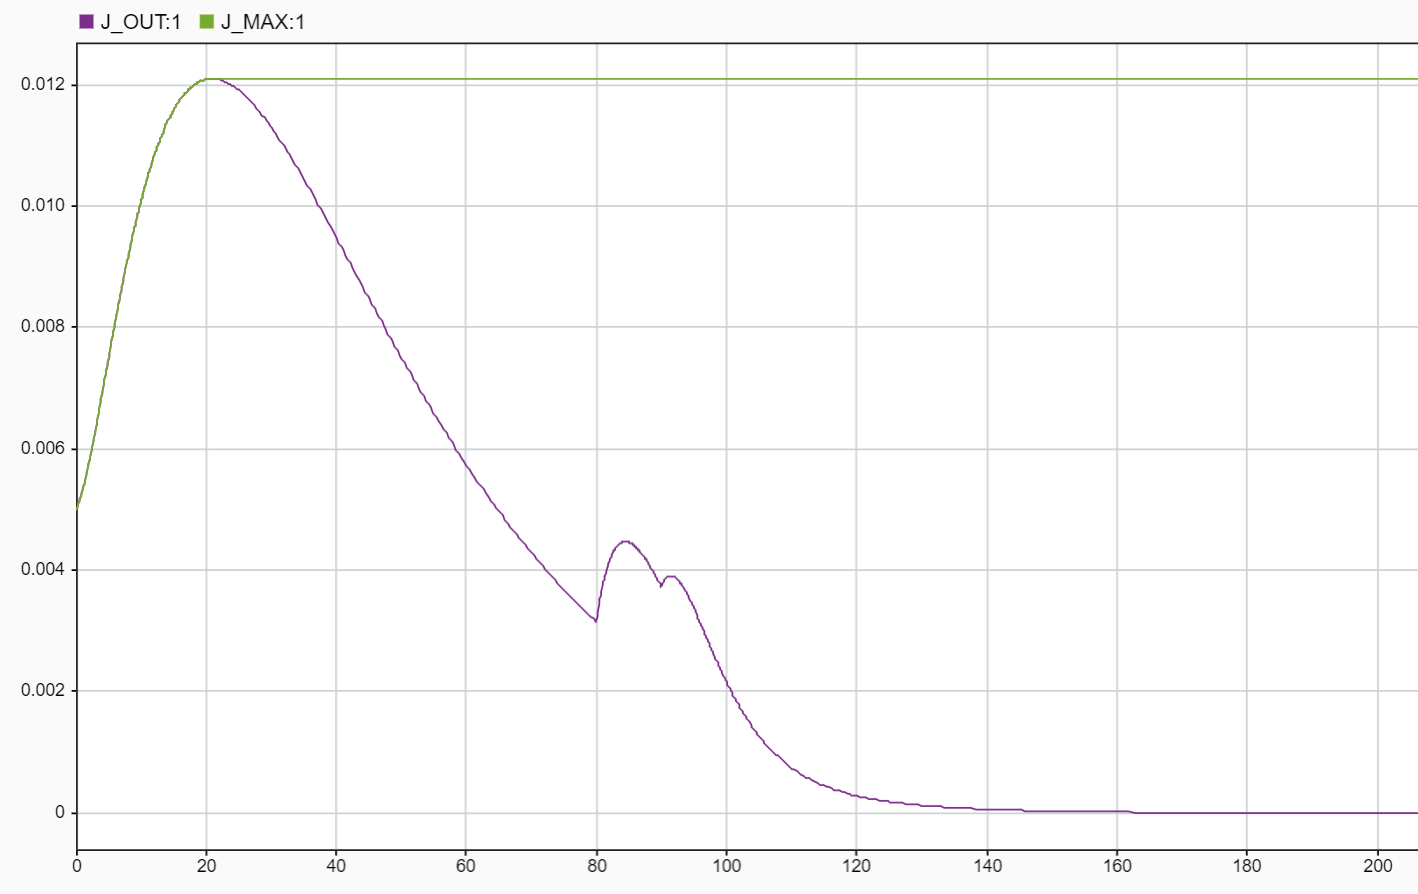
\includegraphics[width=0.7\linewidth]{init_conditions_higher_i} 
\end{center}

Raising the initial value of J to $1\%$ (by subtracting $1\%$ of the population from the S group) did not result in an overload of the hospital system. As shown in the next plot, although the value of J initially starts at the maximum, it decreases since there is not yet a significant percentage of exposed individuals (E) in the population.

\begin{center}
    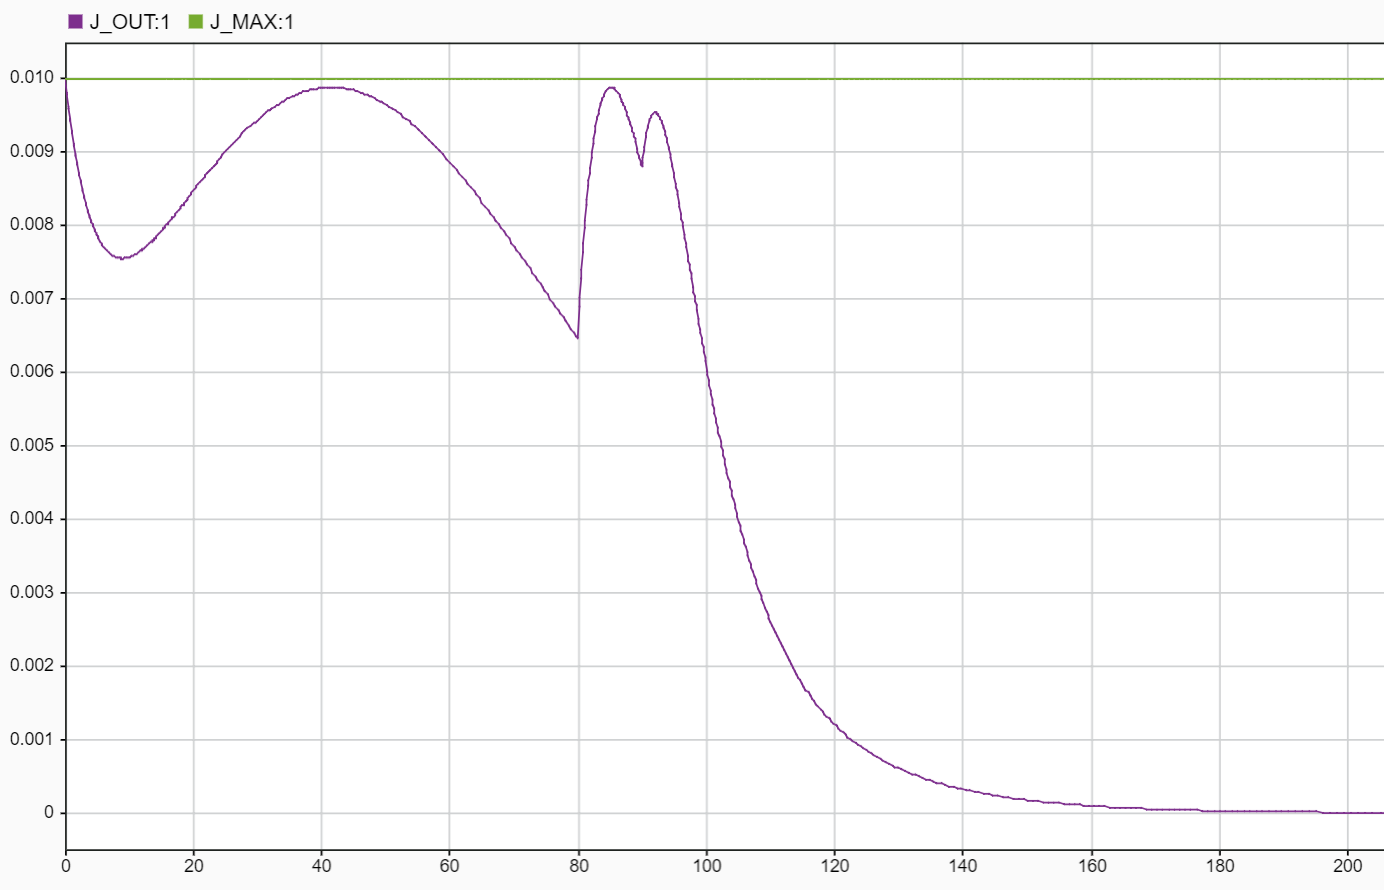
\includegraphics[width=0.7\linewidth]{init_conditions_high_j} 
\end{center}

\newpage

\subsection*{Results}
For different S, E, and I initial conditions, the model will need to be adjusted to control the initial overshoot conditions. In general, it appears that higher percentages in these groups require a stricter mask policy (higher value of u) and vice versa. Additionally, moving a percentage of the population from S, E, I, and J to either R or D will allow for a lower value for u since recovered and dead individuals can no longer be hospitalized due to the virus in this model.

Like before, the effect of raising u results in a more damped response of the number of hospitalizations that ultimately reduces overshoot and a lower peak hospitalization percentage. Therefore, initially raising u to the highest possible value (u=0.9) and reducing it at t=100 after most individuals have either recovered or died would work for the majority of initial conditions.
\end{document}
